\documentclass[notheorems]{beamer}

\usepackage{lipsum}
\usepackage{mathtools}
\usepackage[
  %german,
  %light
]{cknopmpf}


\title{EE3015 \& EE3025 Presentation}
\author{Koidala SURYA Prakash}
\shortauthor{Surya Prakash}
\email[1]{ee18btech11026@iith.ac.in}


%-----------------------------------------------------------------------


\begin{document}
\maketitle

\section{Assignment 1}

\begin{frame}{Assignment 1}{Problem 6.4}


\begin{gather}
     \text{Given   } x(n) = \{ \underset{\uparrow}{1},2,3,4,2,1 \}
         \label{eq:equation0}\\
        y(n) + \frac{1}{2}y(n-1) = x(n) + x(n-2)	
        \label{eq:equation1} \\ 
        \implies   h(n)=\left({\frac{-1}{2}}\right)^nu(n) + \left({\frac{-1}{2}}\right)^{n-2}u(n-2)
        \label{eq:equation2} 
\end{gather}

\begin{block}{Question}
Compute $X(k)$, $H(k)$ and $y(n)$ using FFT and IFFT methods.
\end{block}

\end{frame}


\begin{frame}{Solution}
 Computing y (for N samples) using FFT and IFFT : 
 
\begin{gather}
X = FFT(x)
\label{eq:equation3}\\
H = FFT(h)
\label{eq:equation4}\\
Y = X.H
\label{eq:equation5}\\
y = IFFT(Y) = \frac{1}{N} * FFT(Y^{*})  \{ \texttt{only if y is real} \}
\end{gather}

where $Y^{*}$ = complex conjugate of Y 
\end{frame}

\begin{frame}{Recursive N-point FFT Algorithm   }

    An N-point DFT can be written as : 
\begin{align*}
 X_{k} &=  \sum_{n=0}^{N-1} x(n)e^{-j2\pi kn/N}, \quad k=0,1, \ldots, N-1 \\
       &=  \underbrace{\sum_{m=0}^{N/2 -1} x_{2m}e^{-\frac{j2\pi km}{N/2}}}_\text{ N/2 DFT with even inputs} + W_{N}^k \underbrace{\sum_{m=0}^{N/2 -1} x_{2m+1}e^{-\frac{j2\pi k(m)}{N/2}}}_\text{N/2 DFT with odd inputs}
\end{align*}
where $W_{N} = e^{\frac{-j 2\pi }{N}}$ 


\end{frame}


\begin{frame}{Recursive N-point FFT Algorithm   }

While exploiting symmetry of $W_{N}$ as :

\begin{align}
  W_{N}^{k+N/2} = -W_{N}^k  
\end{align}

We transformed  the  iterative DFT problem  to a Divide-Conquer algorithm as :
\begin{align}
    X_{0\rightarrow \frac{N}{2}-1} = X_{even} + \overline{W}_{N/2}* X_{odd} \\
    X_{\frac{N}{2}\rightarrow N-1} = X_{even} - \overline{W}_{N/2} * X_{odd} 
\end{align}

 $$\overline{W}_{N/2}(i) = W_{N}^i $$;  for i = 0,1,2 ... (N/2) -1 \bigskip\\
\end{frame}


\begin{frame}{Assignment 1}{Problem 6.5}
\textbf{\textcolor{cyan}{Matrix representation of the FFT algorithm}}

An 8-point DFT can be represented as a Matrix product as follows:
$$\overline{X} = \overline{W}\;  \overline{x}$$ 
\begin{equation}
\resizebox{.85\hsize}{!}{
\begin{bmatrix}
X(0) \\X(1) \\X(2) \\X(3) \\X(4) \\X(5) \\X(6) \\X(7) \\
\end{bmatrix}  = 

\begin{bmatrix}
W^{0} & W^{0} & W^{0} & W^{0} & W^{0} & W^{0} & W^{0} & W^{0} \\
W^{0} & W^{1} & W^{2} & W^{3} & W^{4} & W^{5} & W^{6} & W^{7} \\
W^{0} & W^{2} & W^{4} & W^{6} & W^{0} & W^{2} & W^{4} & W^{6} \\
W^{0} & W^{3} & W^{6} & W^{1} & W^{4} & W^{7} & W^{2} & W^{5} \\
W^{0} & W^{4} & W^{0} & W^{4} & W^{0} & W^{4} & W^{0} & W^{4} \\
W^{0} & W^{5} & W^{2} & W^{7} & W^{4} & W^{1} & W^{6} & W^{3} \\
W^{0} & W^{6} & W^{4} & W^{2} & W^{0} & W^{6} & W^{4} & W^{2} \\
W^{0} & W^{7} & W^{6} & W^{5} & W^{4} & W^{3} & W^{2} & W^{1} \\

\end{bmatrix}

\begin{bmatrix}
x(0) \\ x(1) \\ x(2) \\ x(3) \\ x(4) \\ x(5) \\x(6) \\x(7)
\end{bmatrix}

}
\end{equation}

\end{frame}

\begin{frame}
The FFT algorithm decompose $\overline{W}$ into sparse matrices by  permuting $\overline{x}$ in  a  bit-reversed fashion resulting in $\overline{x_{p}}$

\begin{align}
$$\overline{X} = \overline{W3} \; \overline{W2}\;\overline{W1} \; \overline{x_p}$$\newline
\end{align}

\begin{equation}
\resizebox{1\hsize}{!}{
\begin{bmatrix}
X(0) \\X(1) \\X(2) \\X(3) \\X(4) \\X(5) \\X(6) \\X(7) \\
\end{bmatrix}  = 

\begin{bmatrix}
1&.&.&.&W^{0}&.&.&. \\
.&1&.&.&.&W^{1}&.&. \\
.&.&1&.&.&.&W^{1}&. \\
.&.&.&1&.&.&.&W^{1} \\
1&.&.&.&-W^{0}&.&.&. \\
.&1&.&.&.&-W^{1}&.&. \\
.&.&1&.&.&.&-W^{1}&. \\
.&.&.&1&.&.&.&-W^{1} 
\end{bmatrix}

\begin{bmatrix}
1&.&W^{0}&.&.&.&.&.\\
.&1&.&W^{2}&.&.&.&.\\
1&.&-W^{0}&.&.&.&.&.\\
.&1&.&-W^{2}&.&.&.&.\\
.&.&.&.&1&.&W^{0}&.\\
.&.&.&.&.&1&.&W^{2}\\
.&.&.&.&1&.&-W^{0}&.\\
.&.&.&.&.&1&.&-W^{2} 
\end{bmatrix}

\begin{bmatrix}
1&W^{0}&.&.&.&.&.&. \\
1&-W^{0}&.&.&.&.&.&. \\
.&.&1&W^{0}&.&.&.&.\\
.&.&1&-W^{0}&.&.&.&.\\
.&.&.&.&1&W^{0}&.&.\\
.&.&.&.&1&-W^{0}&.&.\\
.&.&.&.&.&.&1&W^{0}\\
.&.&.&.&.&.&1&-W^{0}\\
\end{bmatrix}

\begin{bmatrix}
x(0) \\ x(4) \\ x(2) \\ x(6) \\ x(1) \\ x(5) \\x(3) \\x(7)
\end{bmatrix}

}
\end{equation}

\end{frame}


\begin{frame}{Relation with the butterfly diagram}
 \begin{figure}[!ht]
	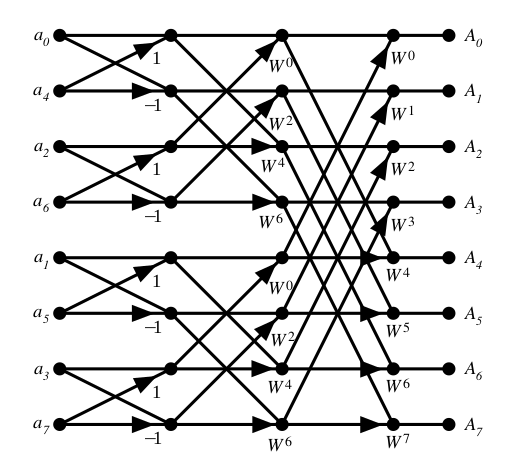
\includegraphics[width=6cm]{figs/butterfly.png}
	\caption{8-point FFT butterfly diagram}
\end{figure}

Ref : Heckbert, P., 1995. Fourier transforms and the fast fourier transform (fft) algorithm. Computer Graphics, 2, pp.15-463.
\end{frame}

\begin{frame}{Time complexity}


Convolution/DFT requires $ N^{2}$ operations $\approx \boldsymbol{O(N^{2})}$.\\
While the same output can be achieved using FFT and IFFT within : 
\begin{equation}
   \underbrace{O(NlogN)}_{\substack{\text{$x \rightarrow X$} \\ {\text{$h \rightarrow H $}}  }} + 
   \underbrace{O(N)}_{\text{$Y = X*H$}} + 
   \underbrace{O(NlogN)}_{\text{$Y \rightarrow y$}} \approx \boldsymbol{O(NlogN)}
\end{equation}

 \begin{figure}[!ht]
	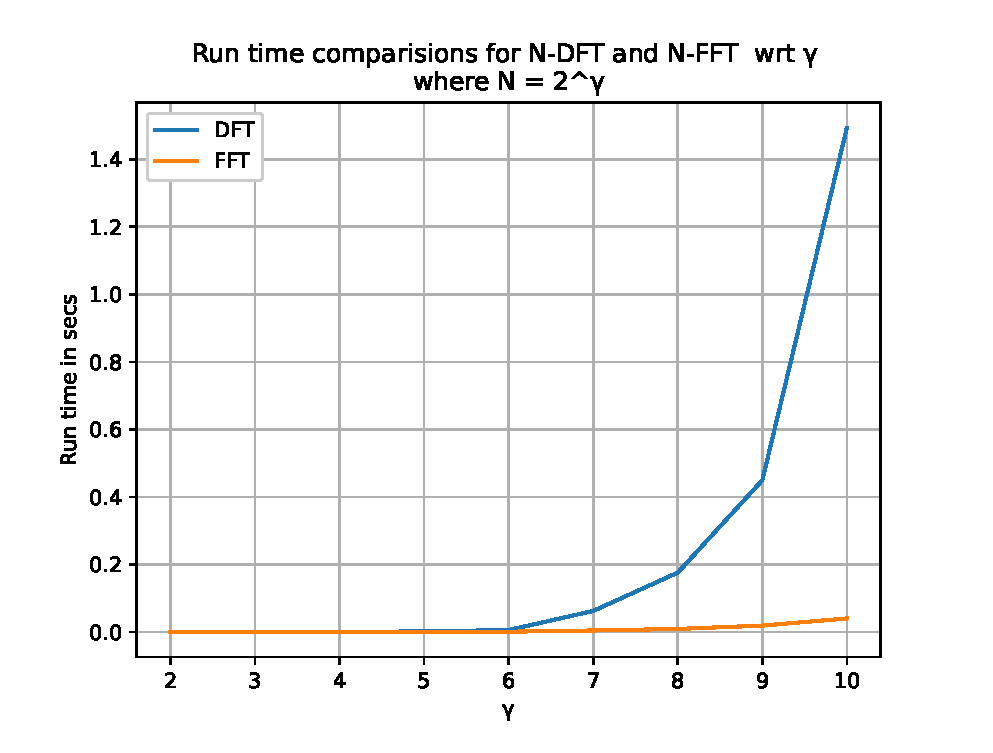
\includegraphics[width=7cm]{figs/dft_vs_fft.eps}
	\caption{Time complexity comparision}
\end{figure}

\end{frame}


\begin{frame}{C vs Python Implementaion}
 \begin{figure}[!ht]
	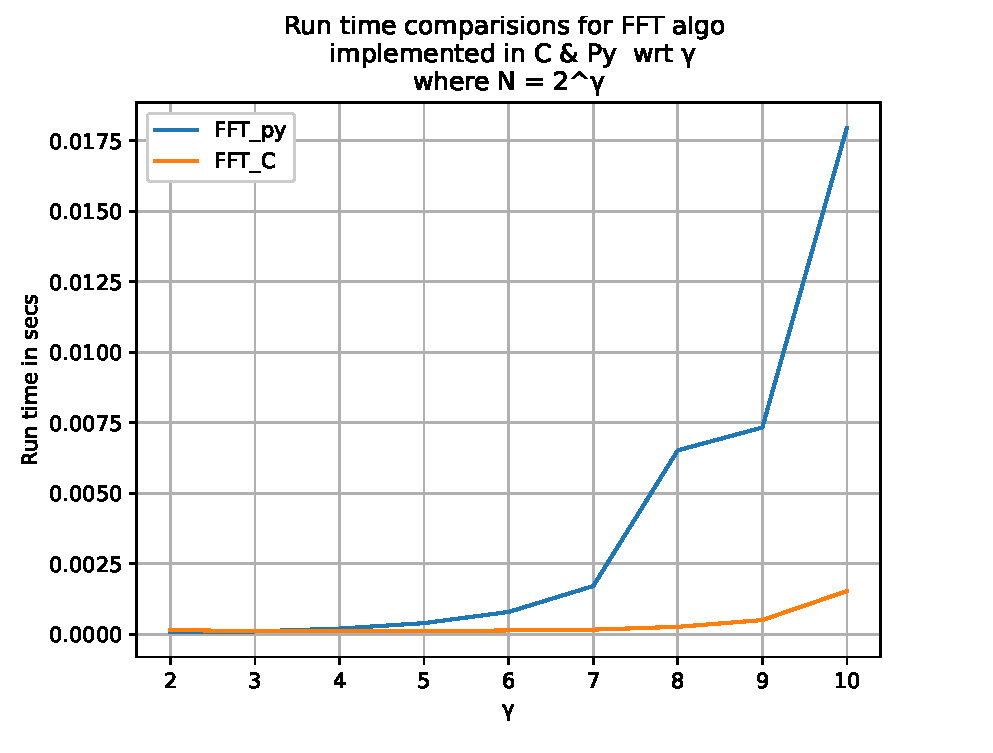
\includegraphics[width=7cm]{figs/fftpy_vs_fftc.eps}
	\caption{Comparing C vs Py implementation}
\end{figure}
\end{frame}
%%%%%%%%%%%%%%%%%%%%%%%%%%%%%%%%%%%%%%%%%%%%%%%%%%%%%%%%%%%%%%%%%%
%%%%%%%%%%%%5     Assignment 02
%%%%%%%%%%%%%%%%%%%%%%%%%%%%%%%%%%%%%%%%%%%%%%%%%%%%%%%%%%%%%%%%%

\section{Assignment 2}

\begin{frame}{Assignment 02}

Design equivalent FIR realizations for filter number 114 with the following specifications.

\begin{columns}
\begin{column}[t]{0.5\textwidth}
\dotfill\\
\texttt{\textcolor{cyan}{Pass band specifications}}\\

$$F_{s} = 48kHz $$
$$F_{p1} = 7.2kHz \; ; F_{p2} = 6kHz $$
$$ \omega_{p1} = 0.3 \pi \; ; \omega_{p2} = 0.25 \pi  $$
$$ \omega_{c}  = 0.275\pi $$

$$\omega_l = \frac{\omega_{p1} - \omega_{p2}}{2} = 0.025 \pi$$

\dotfill
\end{column}\vrule \hfill

\begin{column}[t]{0.5\textwidth}
\dotfill\\

\texttt{\textcolor{cyan}{Stop band specifications}}\\

$$ \texttt{Tolerance:} \delta_1 = \delta_2 = \delta = 0.15 $$
$$ \Delta F = 0.3  kHz \; ; \Delta \omega = 0.0125\pi $$
$$F_{s1} = 7.5Hz \; ; F_{s2} = 5.7kHz $$
$$ \omega_{s1} = 0.3125 \pi \; ; \omega_{s2} = 0.2375 \pi \\ $$

\dotfill
\end{column}
\end{columns}
\end{frame}

\begin{frame}{Designing a low pass equivalent}

\begin{equation}
h_l(n) = \frac{\sin(n\omega_l)}{n\pi}w(n)
\end{equation}

The Kaiser window is defined and computed as :

\begin{align*}
w(n) &= \frac{I_0\left[ \beta N \sqrt{1 - \left(\frac{n}{N}\right)^2} \right]}{I_0(\beta N)},
\indent -N \leq n \leq N, \indent \beta > 0 \nonumber  \\
	&=  0 \hspace{5cm} \mbox{otherwise,}
\end{align*}

Parameters of Kaiser window are : 

$$ A =  -20\log_{10}\delta =  16.478 (< 21) \implies \beta N = 1 $$
$$   N \geq \frac{A-8}{4.57\Delta \omega} = 47.2 \implies chosen \;  N = 100 $$


\end{frame}



\begin{frame}

\begin{columns}
\begin{column}[t]{0.4\textwidth}



\small

\begin{align*}
w(n) &= 1, \indent -100 \leq n \leq 100 \nonumber \\
		&= 0 \hspace{6mm} \mbox{otherwise}
\end{align*}

\texttt {Desired lowpass filter impulse response is }
\begin{align*}
h_{lp}(n) &= \frac{\sin(\frac{n\pi}{40})}{n\pi}  \indent \; ; -100 \leq n \leq 100 \nonumber \\
&= 0, \hspace{2cm} \mbox{otherwise}
\end{align*}

\end{column}

\begin{column}[t]{0.6\textwidth}
\begin{figure}
\label{fig6}
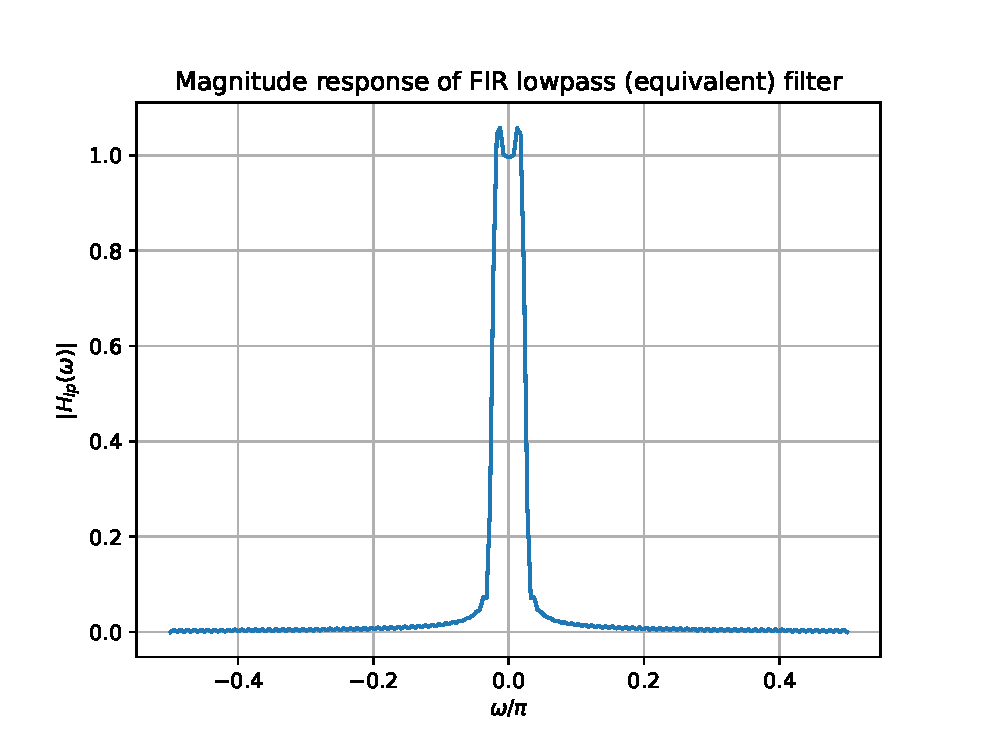
\includegraphics[width = 6.5cm]{figs/FIR_lowpass.eps}
\caption{Magnitude response of the FIR lowpass digital filter } 
\end{figure}
\end{column} 

\end{columns}

\end{frame}

\begin{frame}{ Converting into a causal FIR Bandpass Filter}
A band pass filter can be obtained from a low pass equivalent through the following transformation ...
\small
\begin{equation}
H_{bp}(j\omega) = H_{lp}(j(\omega - \omega_{c})) + H_{lp}(j(\omega + \omega_{c}))
\end{equation}

\begin{equation}
\implies h_{bp}(n) = h_{lp}(n)* 2cos(n\omega_c)
\end{equation}

\begin{figure}
\label{fig7}
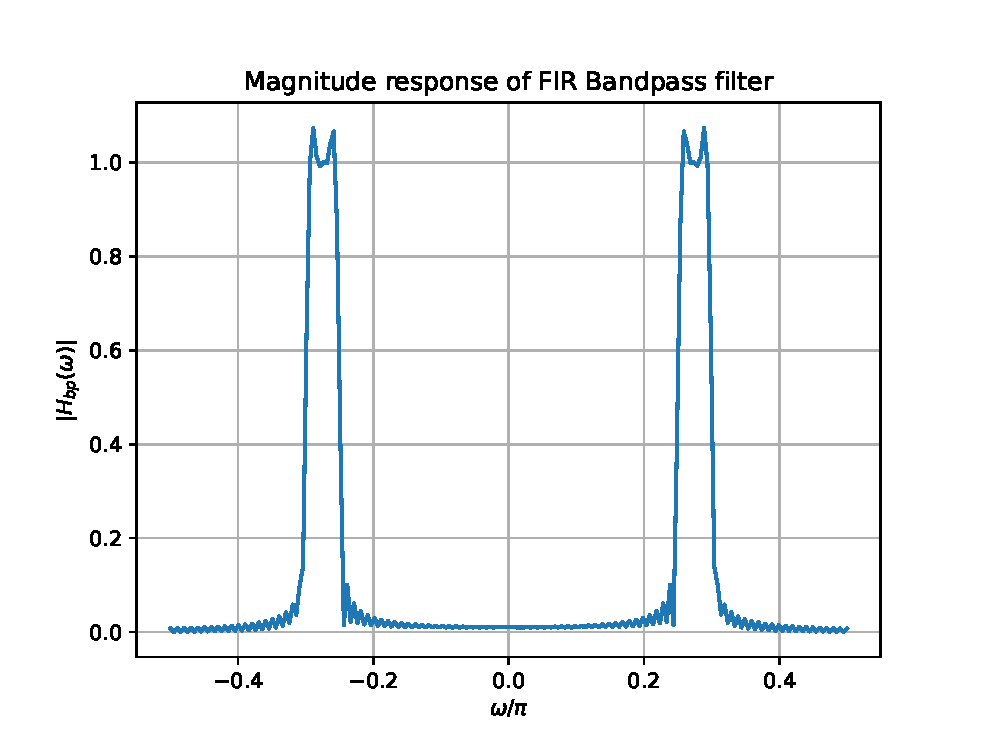
\includegraphics[width = 5.75cm]{figs/FIR_bandpass.eps}
\caption{Magnitude response of the FIR bandpass digital filter } 
\end{figure}

\end{frame}

\begin{frame}

\begin{block}{References}
Heckbert, P., 1995. Fourier transforms and the fast fourier transform (fft) algorithm. Computer Graphics, 2, pp.15-463
\end{block}

\begin{block}{Code \& Reports}
\small
\begin{itemize}

\item Assignment-01\href{https://github.com/Surya291/ACADEMIA/tree/master/IDP_3_2/Asst_01}{\textcolor{cyan} { \; Link }}
\item Assignment-02 \href{https://github.com/Surya291/ACADEMIA/tree/master/IDP_3_2/Asst_02}{\textcolor{cyan} { \; Link }}

\item Beamer template \href{https://github.com/jakobbbb/cknopmpf}{\textcolor{cyan} { \; Link }}

\end{itemize}
\end{block}


  \centering \Huge
  \emph{Thank You !!}


\end{frame}





\end{document}
